% =====================================================================
%  The Limits of Behavioral Early Warning for Copy-Trading Blow-Ups
%  arXiv: q-fin.TR
%  Single author: Syuan Wei Peng (Sean Peng), Mnemox AI
%
%  Standard article class + only arXiv-safe packages.
%  Compile:  pdflatex main ; bibtex main ; pdflatex main ; pdflatex main
% =====================================================================
\documentclass[11pt,a4paper]{article}

\usepackage[utf8]{inputenc}
\usepackage[T1]{fontenc}
\usepackage{lmodern}
\usepackage[margin=1in]{geometry}
\usepackage{amsmath}
\usepackage{amssymb}
\usepackage{booktabs}
\usepackage{graphicx}
\usepackage{xcolor}
\usepackage[numbers,sort&compress]{natbib}
\usepackage{caption}
\usepackage{enumitem}
\usepackage[hidelinks]{hyperref}

\graphicspath{{figures/}}

% --- lightweight helpers (no exotic packages) -------------------------
\newcommand{\fpr}{\mathrm{FPR}}
\newcommand{\Tnull}{T_{0}}
\captionsetup{font=small,labelfont=bf}

\title{\bfseries The Limits of Behavioral Early Warning for\\
Copy-Trading Blow-Ups\\[4pt]
\large A Pre-Registered, Full-Universe On-Chain Study (Hyperliquid)}

\author{Syuan Wei Peng (Sean Peng)\thanks{Mnemox AI. Correspondence:
\texttt{sean@mnemox.ai}. The author thanks Yijia Xiao (UCLA) for the arXiv
endorsement. This is a pre-registered, observational study on the full Hyperliquid
leaderboard universe: the cohort definition, detector, operating point, and claim
gates were frozen in a timestamped commit \emph{before} the sealed test split was
read once (Appendix~\ref{app:op}).}\\
Mnemox AI}

\date{\today}

\begin{document}
\maketitle

% =====================================================================
\begin{abstract}
% ~200 words
A common, rarely-tested assumption behind copy-trading risk controls is that
``behavioral monitoring catches blow-ups'': that a master trader's conduct drifts
\emph{before} the equity damage that wipes out followers. We test this on real
on-chain money over the \emph{full} public Hyperliquid leaderboard---37{,}895
addresses, filtered to 10{,}395 ``master-worth-copying'' accounts, yielding
\textbf{2{,}621 genuine loss-driven idiosyncratic blow-ups} across 48 independent
crash-days. On a model-free panel of 2{,}477 blow-up masters, behavioral drift
leads equity for only \textbf{9\%} (216 masters); \textbf{69\% blow up with no
gradual behavioral signal at all}, and the overall median lead is \emph{negative}
($-8$ days)---when conduct moves, it typically \emph{lags} the equity rather than
leading it. A purpose-built three-axis mixture-SPRT detector, pre-registered with
its operating point frozen on a disjoint tuning split and read once against a
sealed test set, confirms the boundary rather than beating it: it achieves
\emph{chance-level} discrimination (AUC $0.49$) at $2\%$ recall. It does post the
lowest false-positive rate of any method ($0.040$, $\approx\!1.9\times$ below a
leverage tripwire), but at negligible recall that precision is of little practical
use. Behavioral early warning is therefore \emph{not} a viable general safety net
for copy-trading blow-ups: most are sudden, a plain equity / drawdown stop
dominates, and the residual behavioral signal---gradual over-leveraging---precedes
fewer than one blow-up in ten.
\end{abstract}

\medskip
\noindent\textbf{Keywords:} copy trading; behavioral drift; early warning;
sequential testing; mixture SPRT; perpetual futures; on-chain risk; Hyperliquid.

\medskip
\noindent\textbf{JEL / arXiv:} q-fin.TR (Trading and Market Microstructure);
G11, G23, G41.

% =====================================================================
\section{Introduction}
\label{sec:intro}

Copy trading and social trading let retail followers mirror a ``master'' trader's
positions automatically. The arrangement industrializes a single account's risk:
when a master blows up, every follower blows up with them, on the same candle.
Regulators have repeatedly flagged this contagion channel and the asymmetry of
information it creates: a follower sees a headline return and a leaderboard rank,
not the master's moment-to-moment risk-taking
\citep{iosco2025imitative,esma2023copytrading,pelster2019socialtrading}.
The implicit promise of every ``risk score'' and ``copy-stop'' product layered on
top is that \emph{watching how the master trades} gives an earlier, cleaner warning
than watching the equity curve alone.

That promise rests on a load-bearing empirical assumption that is almost never
tested adversarially on real adversarial data: \textbf{behavioral drift precedes
the equity damage.} If a master's conduct degrades gradually---creeping leverage,
abandoned stops, averaging into losers---before the account craters, then a
behavioral monitor buys followers lead-time the equity itself cannot. If instead
most blow-ups are \emph{sudden}---one oversized trade, a gap, or a master who was
always reckless and simply got unlucky---then there is no behavioral runway to
detect, and a plain equity threshold is both simpler and earlier.

We put this assumption on real on-chain money. Hyperliquid is a high-volume
decentralized perpetual-futures venue whose public \texttt{info} API exposes, with
no authentication, every fill, order, and ledger event for any address, plus a
coarse account-value history \citep{hyperliquid2024docs}. This is an unusually
honest laboratory: positions and liquidations are settled on-chain, the
leaderboard is public, and there is no survivorship curation by a broker. We
freeze a leaderboard universe at a fixed date, label blow-ups by a forward-only
equity rule, and ask---first model-free, then with a purpose-built detector---when,
and for whom, behavior actually leads equity.

\paragraph{Our contribution is a clean negative.}
\begin{enumerate}[leftmargin=1.4em,itemsep=2pt]
  \item \textbf{The boundary (the headline).} On 2{,}477 real idiosyncratic
        blow-up masters, behavioral drift leads equity for only $\approx$9\%; 69\%
        are sudden; the overall median lead is \emph{negative}. The popular
        ``behavioral monitoring catches blow-ups'' assumption is false as a general
        law, including in an earlier, scaled-cohort version of this project, whose
        more favorable numbers this full-universe run overturns.
  \item \textbf{A pre-registered detector that confirms it.} A three-axis
        mixture-SPRT detector, frozen on a disjoint tuning split and read once
        against a sealed test set, achieves \emph{chance-level} discrimination
        (AUC $0.49$) at $2\%$ recall: the behavioral machinery cannot rank a
        soon-to-blow-up master above a stable one. It does attain the lowest
        false-positive rate of any method ($\approx 1.9\times$ below a leverage
        tripwire), a real but, at this recall, inconsequential property.
  \item \textbf{What little survives is exposure.} Among the few masters that do
        drift early, the trigger is almost always the exposure (leverage) axis, not
        discipline or tilt---but it precedes fewer than one blow-up in ten, and our
        on-chain leverage proxy is coarse, so we do not over-read the mechanism.
\end{enumerate}

We are explicit about epistemic status. This is a \emph{pre-registered},
observational study on the \emph{full} leaderboard universe: the cohort definition,
detector form, operating point, and claim gates were frozen in a timestamped commit
\emph{before} the sealed test split was read (Appendix~\ref{app:op}). It overturns
an earlier exploratory, scaled-cohort version that had reported a usable
high-precision detector; the contamination that inflated that result---withdrawal
-driven equity craters mislabeled as trading blow-ups---is removed here by a
loss-confirmed labeling rule (Section~\ref{sec:data}). Honesty about where
behavioral early warning works \emph{and}, mostly, where it does not is the point of
the paper, not a caveat to it.

% =====================================================================
\section{Related work}
\label{sec:related}

\paragraph{Copy / social trading and its risks.}
Social-trading platforms have been studied mostly from the follower's behavioral
side---herding, the disposition effect amplified by visible reputation, and the
hazards of mirroring leveraged strategies
\citep{pelster2019socialtrading,barber2000trading}. Supervisory bodies have issued
explicit warnings about copy trading and ``finfluencer''-driven retail
participation, stressing the information asymmetry between the copied master and
the copier \citep{iosco2025imitative,esma2023copytrading}. Commercial copy
desks operationalize this with proprietary ``risk scores'' and automatic
copy-stops; the canonical example is a forex copy-trading risk guard that monitors
a master and can pause copying. Such systems are typically closed, forex-centric,
and---critically---unvalidated in public against the alternative of simply watching
equity. Our detector targets the same job (drift / behavioral risk intelligence for
a broker or copy desk) but is vendor-neutral, on-chain, and reported with its
false-positive rate alongside its lead-time.

\paragraph{Changepoint and statistical process control.}
Detecting a shift in a stream is classical. The cumulative sum (CUSUM) chart and
its SPC relatives detect a step change in a monitored statistic
\citep{page1954cusum,montgomery2009spc}; Bayesian Online Changepoint Detection
(BOCPD) maintains a run-length posterior \citep{adams2007bocpd}. Our per-axis test
is a sequential probability ratio test \citep{wald1945sprt} in its mixture form
(mSPRT), which is ``always valid''---it controls error under continuous monitoring
and optional stopping, exactly the peeking problem that arises when an alarm is
checked every bucket \citep{johari2017peeking}. We compose three axes with a
Holm correction \citep{holm1979simple} and shrink each axis's self-baseline toward
a universe prior in James--Stein fashion \citep{james1961stein}.

\paragraph{Behavioral / concept drift.}
``Drift'' in a trader is a special case of concept drift---the statistical
properties of a stream changing over time \citep{gama2014concept}. The
machine-learning literature emphasizes detecting and adapting to drift; we instead
ask the prior question of whether a financially-meaningful drift even exists ahead
of the outcome it is supposed to predict.

\paragraph{Equity thresholds vs.\ behavioral detectors: reframed.}
In earlier internal work on self-monitoring trading agents we found that a simple
maximum-drawdown stop on the equity curve outperformed a CUSUM behavioral detector
for cutting losses---a result mirrored in the drawdown-control literature
\citep{magdon2004maxdd}. We previously read this as a defeat for behavioral
methods. The present study reframes it correctly: \emph{equity-threshold methods
win in general because most blow-ups are sudden} (Section~\ref{sec:results}). When
the damage arrives without a gradual behavioral antecedent, nothing beats reading
the damage directly. Behavioral detectors could only add value within the gradual
subclass, and that subclass turns out to be both small (under one blow-up in ten)
and, even with a pre-registered detector, not separable from stable masters above
chance (Section~\ref{sec:results}). The reframing sharpens the negative rather than
rescuing the method: equity wins not by a narrow margin but because the behavioral
runway a detector would need is usually not there.

\paragraph{Methodological hygiene.}
Performance studies in finance are notoriously fragile to survivorship bias
\citep{brown1991survivorship}, multiple testing and backtest overfitting
\citep{harvey2015backtesting}, and clustered dependence. We address these with a
frozen-at-$\Tnull$ universe (no survival filter), a strict tuning/test split with
the operating point chosen off the test data, and event-clustered bootstrap
inference \citep{efron1986bootstrap,cameron2008clusterboot} that resamples
crash-days rather than masters.

% =====================================================================
\section{Data}
\label{sec:data}

\paragraph{Source.}
All data come from the public Hyperliquid \texttt{info} API
\citep{hyperliquid2024docs}, which requires no authentication: per-address fills
(\texttt{userFills}, carrying a \texttt{liquidation} flag), orders
(\texttt{historicalOrders}, including trigger / reduce-only metadata), ledger
updates (\texttt{userNonFundingLedgerUpdates}, including margin top-ups and
withdrawals), and a coarse account-value history (\texttt{portfolio}). Requests are
throttled ($\geq 0.4$\,s spacing) with retry on rate-limit, and raw responses are
archived for reproducibility (Appendix~\ref{app:repro}).

\paragraph{Frozen universe.}
To kill survivorship bias we freeze the universe at $\Tnull = $ 2025-06-01 UTC and
look forward to a window end of 2026-04-30 UTC ($\approx$11 months). The universe
is a leaderboard snapshot filtered to addresses with a pre-$\Tnull$ peak perpetual
account value $\geq \$25{,}000$ (a ``master worth copying'' floor that removes
dust) and at least two pre-$\Tnull$ equity points. Selection uses \emph{only}
information available at $\Tnull$; no outcome (survival) filter is applied. We
process the \emph{entire} leaderboard---37{,}895 addresses---and retain the
\textbf{10{,}395} that clear the floor. Crucially, the filter is on the
\emph{pre-}$\Tnull$ \emph{peak}, not on the current account value: masters who have
since blown up below \$25k are kept rather than silently dropped, which is the
selection error that would otherwise hide exactly the events we study.

\paragraph{Labeling (forward-only, loss-confirmed).}
A master is labeled a blow-up by a forward-only, \emph{loss-confirmed} rule
(Appendix~\ref{app:rule}): scanning forward from $\Tnull$, the first peak-to-trough
drawdown exceeding 70\% with no recovery to 80\% of the prior peak within 30 days
\emph{whose cumulative-PnL drop is at least half the equity drop}. The
loss-confirmation is not cosmetic. At $\Tnull = $ 2025-06-01, \textbf{65\% of naive
equity-only craters are withdrawals, not losses} (median PnL-to-equity-drop ratio
$0.21$): the account value falls because the master moved capital out, not because
trading lost it. A withdrawal crater therefore resets the running peak and the scan
continues, so the labeled time is the first genuinely \emph{loss-driven}
account-death, whenever it occurs. (An earlier scoping pass at a later $\Tnull$ had
found most craters already loss-confirmed; that does not hold at our frozen date,
which is why the filter is enforced \emph{inside} the labeler rather than as an
afterthought.) Among the retained blow-ups the median loss-to-equity ratio is
$1.0$. The rule never looks past the trigger time, so a label cannot leak future
information into the detection window.

\paragraph{Idiosyncratic vs.\ market-event blow-ups.}
A market-wide dump synchronizes many masters on the same UTC day; such days are not
``predict the blow-up'' events but common-shock events. We tag a UTC day as a
\emph{market-event} day when $\geq 3\%$ of the active universe craters on it, and
separate those blow-ups from idiosyncratic ones. This yields \textbf{2{,}621
idiosyncratic blow-ups across 48 independent crash-days}, with the market-event
days (2025-06-04, 2025-06-11, 2025-10-15) tagged and held out of the idiosyncratic
analysis. The effective sample size for inference is the number of independent
crash-day clusters, not the raw blow-up count---hence the event-clustered
statistics in Section~\ref{sec:method}.

\paragraph{Behavioral sub-cohort.}
Equity labeling needs one cheap call per address; the full behavioral trajectory
(fills, orders, ledger) is expensive, so we pull it only for a labeled sub-cohort.
This \emph{behavioral sub-cohort} comprises \textbf{3{,}455 masters (2{,}482
blow-up / 973 stable)}: the idiosyncratic blow-ups whose complete behavioral
trajectory could be fetched within the rate-limited collection window (2{,}482 of
the 2{,}621 labeled; the remainder timed out against the fill-history cap and the
API throttle), plus a seed-fixed matched stable sample, each with a full trajectory.
An address-hashed split assigns 1{,}405 masters to tuning, 656 to validation, and a
\emph{sealed} test set of 1{,}394 (990 blow-up / 404 stable). The operating point is chosen on the tuning split
alone; all Section~\ref{sec:results} numbers are computed on the sealed test set,
read exactly once after the detector was frozen (Appendix~\ref{app:op}).

\paragraph{The 10k-fill-cap selection line.}
Hyperliquid's fill history is capped at the most recent $\approx$10{,}000 fills per
address. For very high-frequency masters this window does not reach back to
$\Tnull$, so a pre-$\Tnull$ behavioral baseline cannot be built from fills. Rather
than drop these masters (which would bias toward low-frequency traders---a
disclosed selection effect), we estimate each master's baseline from its
\emph{earliest in-observation healthy segment} (Section~\ref{sec:method}). We name
this line explicitly because it biases the baseline toward the in-window early
period and we report the fraction affected.

\paragraph{Ethics and pseudonymization.}
All addresses are public pseudonymous on-chain identifiers; no personal identity is
collected, inferred, or published. We report only aggregate statistics; the single
case study (Section~\ref{sec:mechanism}) uses a de-identified trajectory and is
excluded from all inferential claims. No trading is performed and no capital is at
risk; the study is purely observational on already-public ledger data.

% =====================================================================
\section{Method}
\label{sec:method}

\subsection{Three orthogonal behavioral axes}
We summarize a master's order flow on three volatility-normalized axes, each chosen
so that a deteriorating master moves it in a known sign:
\begin{description}[leftmargin=1.6em,itemsep=2pt]
  \item[Exposure ($\uparrow$ is worse).] Leverage, notional growth, and trade
        size-in-sigma (size scaled by the realized volatility of the traded
        instrument). Captures gradual over-leveraging.
  \item[Discipline ($\downarrow$ is worse).] Stop-attach rate, reduce-only rate,
        and holding time. Captures the abandonment of risk controls.
  \item[Tilt ($\uparrow$ is worse).] Margin top-ups, adding-into-losers, and
        trade-rate spikes. Captures emotional / revenge trading.
\end{description}
Each raw primitive is computed per time bucket (4-hour buckets in the reported
configuration) from the trajectory.

\subsection{Early-window self-baseline with shrinkage}
Because the fill cap denies many masters a pre-$\Tnull$ baseline
(Section~\ref{sec:data}), each axis is $z$-scored against an \emph{early-window
self-baseline}: the master's first $\approx$20\% in-observation buckets, restricted
to a still-healthy regime (equity $\geq 90\%$ of running peak and before sustained
drift). Masters already drifting at window start have no clean baseline and are
flagged; the early-baseline robustness is the subject of a stability accounting we
report below. To stabilize small-sample baselines we shrink each master's
per-axis location toward a tuning-split universe distribution by James--Stein
shrinkage \citep{james1961stein} with intensity $\kappa$.

\subsection{Per-axis mixture-SPRT and composite alarm}
On each axis we run a one-sided mixture sequential probability ratio test
\citep{wald1945sprt,johari2017peeking} in the deterioration direction, with
per-axis level $\alpha = 0.01$. The mSPRT is ``always valid'': checking it every
bucket does not inflate the error rate, which is essential because an alarm is, by
construction, monitored continuously \citep{johari2017peeking}. The composite alarm
is a Holm-corrected \citep{holm1979simple} min-gate across the three axes,
\emph{sustained} for $M$ consecutive buckets:
\begin{equation}
\text{alarm}_t \;=\; \mathbf{1}\!\left[
\text{Holm}\!\big(p^{\text{exp}}_t, p^{\text{disc}}_t, p^{\text{tilt}}_t\big)
\text{ rejects for } M \text{ consecutive buckets}\right].
\end{equation}

\subsection{Guard band (anti-label-leakage)}
Exposure and tilt are mechanically coupled to equity, so an ``early'' alarm fired
\emph{after} the damage has begun would be a self-fulfilling label leak. We
therefore impose a guard band: an alarm counts as a genuine early warning only
while equity $\geq 70\%$ of the running peak \emph{and} strictly before the first
liquidation fill. The baseline-estimation segment (earliest healthy buckets) and
the counted-alert region (up to 70\%-of-peak / first liquidation) are thereby
separated in time.

\subsection{Baselines}
We compare against three non-trivial early tripwires, all run under the
\emph{same} guard band so the comparison is apples-to-apples:
\begin{description}[leftmargin=1.6em,itemsep=2pt]
  \item[B1 --- leverage-p90 tripwire.] Fire when leverage exceeds the master's own
        90th percentile.
  \item[B2 --- drawdown-velocity.] Fire on accelerating drawdown velocity.
  \item[B3 --- leverage-up-and-add.] Fire when leverage rises while the master adds
        into a losing position.
\end{description}
The central methodological point: \textbf{comparing lead-time without also
reporting FPR is meaningless when a baseline near-always-fires.} A tripwire that
alerts on essentially every master will trivially ``lead'' every blow-up by a long
margin while being useless in deployment. We therefore report, for every method,
the full triple $(\fpr,\ \text{recall},\ \text{lead})$ on the stable and blow-up
cohorts jointly.

\subsection{Operating-point selection (no test snooping)}
The detector has free knobs (sustain $M$, shrinkage $\kappa$, threshold $\tau$,
bucket size). We choose the operating point \emph{only} on the tuning split: among
grid points with tuning-split stable-FPR $\leq 0.10$ we take the highest-recall
configuration, breaking ties by the longest tuning lead. This selects
$M=3$, $\kappa=7$, $\tau=0.3$, 4-hour buckets, 20-bucket burn-in
(Appendix~\ref{app:op}), which---together with the detector form and the claim
gates---was frozen in a timestamped commit \emph{before} the sealed test split was
read. Every number in Section~\ref{sec:results} is then computed on that sealed
test set, read exactly once. We note that $\kappa$ is effectively inert here
because the self-baseline and the universe prior nearly coincide on-chain
(Section~\ref{sec:discussion}); its frozen value carries no signal.

\subsection{Event-clustered inference}
Blow-ups cluster in time: a handful of crash-days produce many of them, so masters
are not independent observations. All confidence statements resample the
\emph{crash-day clusters} (not the masters), with 5{,}000 bootstrap replicates
\citep{efron1986bootstrap,cameron2008clusterboot}, and we report the effective
number of independent clusters as the true power unit. Leave-one-event-out
robustness is computed analogously.

% =====================================================================
\section{Results}
\label{sec:results}

\subsection{Claim 1 --- the boundary: behavior does not generally lead equity}
\label{sec:boundary}

We first test the load-bearing assumption \emph{model-free}, with no detector. For
each of 2{,}477 real idiosyncratic blow-up masters (those with $\geq$20 behavioral
buckets) we mark $T_{\text{behavior}}$, the first clear degradation versus the
master's own early-window baseline (leverage up, loser-adding, stop-rate down), and
$T_{\text{equity}}$, the first drop below 90\% of peak. The lead is
$T_{\text{equity}} - T_{\text{behavior}}$.

The result is the paper's headline negative (Figure~\ref{fig:boundary}). Behavior
leads equity for only \textbf{216 of 2{,}477 ($\approx$9\%)} masters. Fully
\textbf{69\% blow up with no gradual behavioral signal at all}---they are sudden:
one outsized trade, a gap, or a master who was aggressive throughout with no
``drift'' to detect. Over the cases where both timestamps exist, the median lead is
\emph{negative} (\textbf{$-8$ days}): when behavior moves at all, it more often
\emph{lags} the equity than leads it. Only in the minority right tail is there real
runway---there the median lead is $\approx$\textbf{13 days} (IQR 7.3--24.5\,d), and
it is almost entirely an exposure phenomenon (\textbf{215 of 216} are carried by the
leverage axis, not discipline or tilt).

\begin{figure}[t]
  \centering
  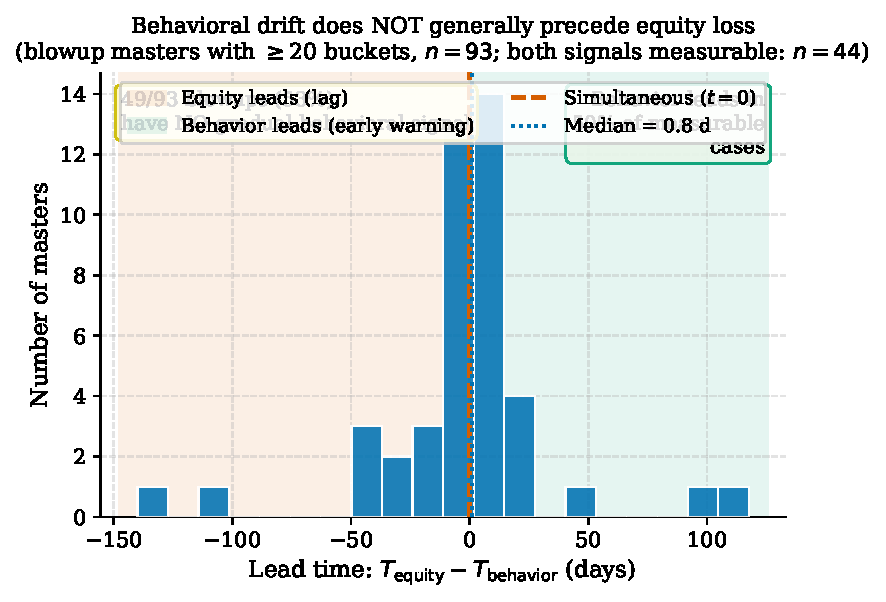
\includegraphics[width=0.82\linewidth]{fig1_boundary.pdf}
  \caption{\textbf{The boundary (Claim 1).} Distribution of the behavior-minus-equity
  lead over the 762 of 2{,}477 idiosyncratic blow-up masters for which both timestamps
  are measurable (model-free, no detector); the remaining 1{,}706 show no gradual
  behavioral signal and cannot be placed on this axis. The mass at and below zero shows
  that behavioral drift does \emph{not} generally precede equity damage: only
  $\approx$9\% of all blow-ups have a positive lead (216 of 2{,}477), 69\% are sudden,
  and the median lead over the measurable cases is \emph{negative} ($\approx-8$\,d).
  The thin right tail is the gradual-leverage minority ($\approx$13-day median lead).}
  \label{fig:boundary}
\end{figure}

The implication is unambiguous: \emph{behavioral monitoring is not a general
early-warning solution for copy-trading blow-ups.} A behavioral detector that
assumes gradual, sustained drift cannot help with the majority of blow-ups, and a
plain equity threshold will fire as early or earlier on the sudden ones. This is
the boundary; the rest of the paper lives inside it.

\subsection{Claim 2 --- the pre-registered detector confirms the boundary}
\label{sec:fair}

A purpose-built behavioral detector might still beat the crude model-free rule. It
does not. On the sealed test set (990 blow-up / 404 stable), with every method under
the same guard band and the detector at its frozen operating point ($M=3$,
$\kappa=7$, $\tau=0.3$, 4-hour buckets), the three-axis mixture-SPRT achieves
\emph{chance-level} discrimination: its continuous drift-evidence score separates
blow-up from stable masters with $\mathrm{AUC}=0.49$ (event-clustered 95\% CI lower
bound $0.47$), and as a binary alarm it fires early on only $2\%$ of blow-ups. The
full $(\fpr,\ \text{recall},\ \text{lead})$ triple for each method is in
Table~\ref{tab:fair} and Figure~\ref{fig:fpr}.

\begin{table}[t]
  \centering
  \caption{\textbf{Fair held-out comparison (Claim 2).} 990 blow-up / 404 stable,
  the \emph{sealed} test set; operating point frozen on a disjoint tuning split
  before the test was read. FPR is measured on stable masters; recall is the
  fraction of blow-ups with a guard-banded early alarm; lead is the median
  alarm-to-crater time among caught blow-ups. The detector posts the lowest FPR
  ($\approx 1.9\times$ below B1) but at only $2\%$ recall, and its $\mathrm{AUC}=0.49$
  is at chance: low FPR with negligible recall is not a usable detector. The
  baselines' longer ``leads'' are a fire-on-everything artifact---they alert on
  17--23\% of \emph{stable} masters.}
  \label{tab:fair}
  \small
  \setlength{\tabcolsep}{5pt}
  \begin{tabular}{@{}lccccl@{}}
    \toprule
    Method & FPR $\downarrow$ & Recall $\uparrow$ & Median lead & FP / 404 & Note \\
    \midrule
    \textbf{Detector (mSPRT, 3-axis)} & \textbf{0.040} & 0.021 & 49 d & 16 & lowest FPR; chance AUC \\
    B1 \;leverage-p90 tripwire        & 0.074 & 0.105 & 52 d & 30 & $1.9\times$ FPR, $5\times$ recall \\
    B2 \;drawdown-velocity            & 0.225 & 0.227 & 70 d & 91 & fires widely \\
    B3 \;leverage-up-and-add          & 0.171 & 0.153 & 72 d & 69 & fires widely \\
    \bottomrule
  \end{tabular}
\end{table}

\begin{figure}[t]
  \centering
  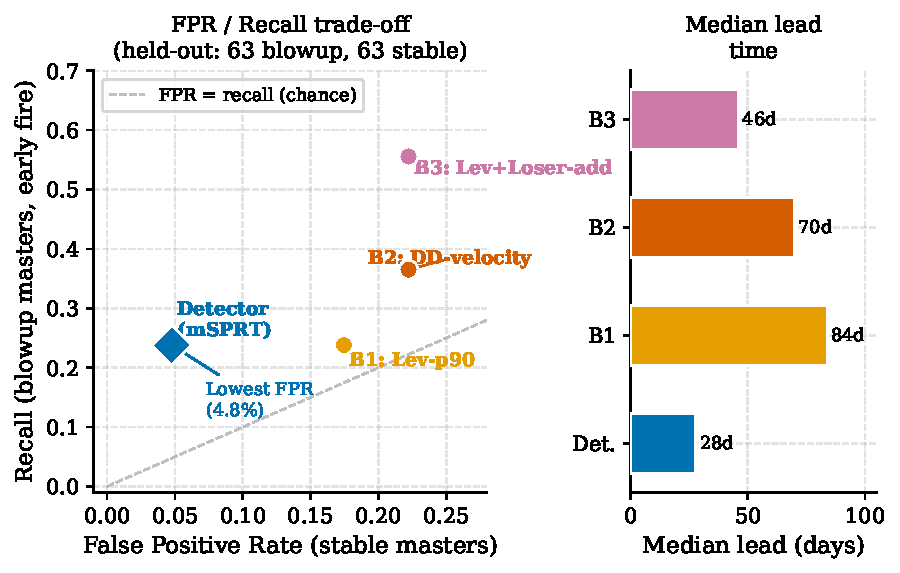
\includegraphics[width=0.72\linewidth]{fig2_fpr_recall.pdf}
  \caption{\textbf{Fair comparison in FPR--recall space (Claim 2).} Each method is a
  point; lower-right is better. The detector sits at the far left (FPR 0.040) but
  near the floor (recall 0.021): the lowest false-alarm rate, almost no coverage,
  and AUC at chance. B1 buys $\approx 5\times$ the recall at $\approx 1.9\times$ the
  FPR; B2/B3 buy more recall only by alerting on 17--23\% of stable masters. Reading
  lead-time without the FPR axis (Table~\ref{tab:fair}) would reward the
  fire-on-everything baselines for an artifact.}
  \label{fig:fpr}
\end{figure}

Three readings follow.
\begin{enumerate}[leftmargin=1.4em,itemsep=2pt]
  \item \textbf{Lowest FPR, but it buys nothing.} The detector false-alarms on 16 of
        404 stable masters ($\fpr = 0.040$) versus 30--91 for the baselines
        ($\fpr = 0.074$--$0.225$)---the lowest by $\approx 1.9\times$. In isolation
        that precision is attractive; paired with $2\%$ recall it means the detector
        is silent on essentially every blow-up that matters.
  \item \textbf{Chance-level discrimination.} The continuous drift-evidence score
        ranks blow-up above stable masters no better than a coin
        ($\mathrm{AUC}=0.49$, event-clustered CI lower bound $0.47$). The behavioral
        signal does not separate the two populations---the pre-registered
        confirmation of Claim 1.
  \item \textbf{The baselines' ``leads'' are an artifact.} B2 and B3 post longer
        median leads (70 d, 72 d) and higher recall only by firing on 17--23\% of
        \emph{stable} masters---near-always-firing. Lead-time read without FPR rewards
        exactly this pathology; with FPR shown, the artifact is plain.
\end{enumerate}

The conclusion is blunt: the detector does \textbf{not} discriminate. Its $2\%$
recall and chance-level AUC make it silent on essentially all blow-ups, and the one
property it owns---a low false-positive rate---is worthless without coverage. This
is the Claim-1 boundary, confirmed by the very machinery built to beat it.

\subsection{Lead-time, where it exists}
\label{sec:leadtime}

Among the minority of blow-ups that \emph{do} show an early behavioral signal, the
lead can be long. Figure~\ref{fig:lead} plots the model-free behavior-minus-equity
lead over the 216 masters with a positive value: a median of $\approx$13 days
(IQR 7.3--24.5\,d), right-skewed, some masters slowly over-leveraging for months
before the crater. This is the most that can be said for behavioral early warning,
and it must be read with its denominator---it is conditioned on the $\approx$9\% of
blow-ups that drift at all. The detector, on the $2\%$ it fires on, shows a
similarly long median ($\approx$49 days); but conditioning on $2\%$ coverage makes
that number a curiosity, not a value proposition.

\begin{figure}[t]
  \centering
  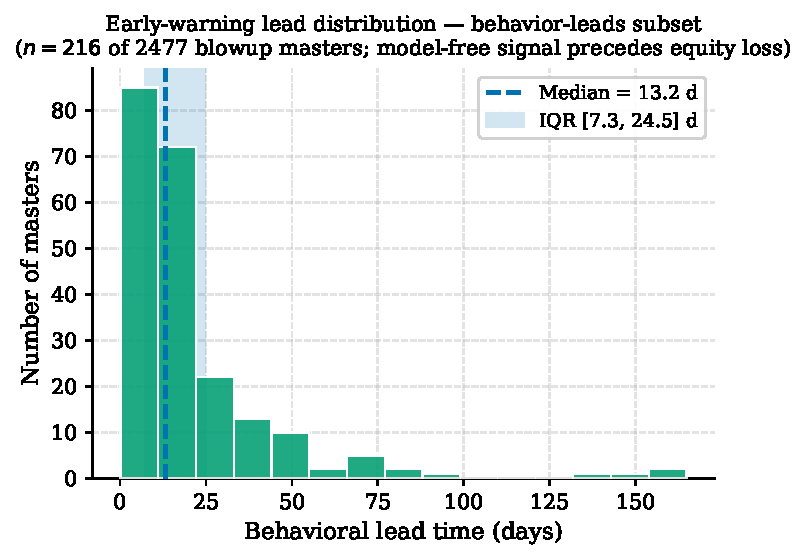
\includegraphics[width=0.72\linewidth]{fig3_leadtime.pdf}
  \caption{\textbf{Lead-time, where it exists (Claim 2).} Model-free
  behavior-minus-equity lead over the 216 idiosyncratic blow-up masters with a
  \emph{positive} lead. Median $\approx$13 days, right-skewed. Long where it
  exists---but conditioned on the $\approx$9\% of blow-ups that show any gradual
  signal; it is silent on the rest.}
  \label{fig:lead}
\end{figure}

\subsection{Claim 3 --- what little survives is exposure}
\label{sec:mechanism}

Which axis carries what signal there is? Almost entirely \textbf{exposure}: in the
model-free boundary analysis, 215 of the 216 behavior-leads masters are triggered by
the leverage axis rather than by discipline (stop-attach, reduce-only) or tilt
(margin top-ups, loser-adding). Two caveats keep this from being a clean
``mechanism.'' First, it describes only the $\approx$9\% gradual minority, not
blow-ups at large. Second, our on-chain leverage signal is a coarse,
volatility-normalized order-flow proxy---not reconstructed account leverage---and the
discipline and tilt primitives are sparse and noisy in public fills, so the
dominance of exposure may partly reflect what is cleanly \emph{measurable} on-chain
rather than a behavioral truth. We therefore report exposure as the surviving
correlate, not as a validated causal channel, and omit a single-master case study
that the noisy leverage proxy cannot support responsibly.

% =====================================================================
\section{Discussion}
\label{sec:discussion}

\paragraph{Why equity beats behavior.}
Equity thresholds win (Section~\ref{sec:related}) \emph{because} most blow-ups are
sudden (Claim 1) and because, even among the gradual minority, a detector
pre-registered and read on a sealed test cannot rank them above stable masters at
better than chance (Claim 2). Our earlier internal reading---``drawdown stops beat a
behavioral CUSUM, so behavioral methods lose''---turns out to have been right, for
the right reason, on a far larger and cleaner sample: when the damage arrives with no
gradual antecedent, nothing beats reading the damage directly, and the antecedent is
usually absent. The conditional that survives is narrow---watch the equity; a
behavioral layer earns its place only if one can first define, causally and ahead of
time, the small subclass that drifts.

\paragraph{Implications for copy-desk risk controls.}
The practical message is deflationary. A behavioral overlay that fires on $2\%$ of
blow-ups and ranks them at chance does not earn its place as a general early-warning
layer, however low its false-positive rate. A broker or copy desk is better served
by a plain equity / drawdown stop, which catches the sudden majority directly and at
least as early. The $4\%$ false-positive rate we measure is real and would matter
\emph{if} it came with usable recall; it does not, so it does not rescue the
approach. Behavioral monitoring is, at most, a narrow complement for a
gradual-leverage subclass that is too small, and too hard to define ahead of time,
to anchor a product.

\paragraph{Honest limitations.}
We foreground these because they bound every claim above.
\begin{itemize}[leftmargin=1.4em,itemsep=2pt]
  \item \textbf{Near-zero recall.} The detector fires early on $\approx$2\% of
        blow-ups and discriminates at chance (AUC $0.49$). It is not a general
        copy-trading safety net and must not be sold as one.
  \item \textbf{Coarse on-chain proxies.} The leverage signal is a
        volatility-normalized order-flow statistic, not reconstructed account
        leverage; discipline (stop-attach, reduce-only) and tilt (top-ups,
        loser-adding) rely on sparse, partly opaque public-fill metadata. The
        dominance of the exposure axis may partly reflect what is cleanly measurable
        rather than a behavioral truth.
  \item \textbf{Labeling choices.} Blow-ups are equity-drawdown events with a
        loss-confirmation filter; the $70\%$ threshold, the $0.5$ PnL-to-equity ratio,
        and the early-window self-baseline are defensible but not unique. Robustness
        reruns over the drawdown threshold are noted in Appendix~\ref{app:rule}.
  \item \textbf{Post-hoc subclass.} The ``gradual-leverage'' subclass is identified
        from observed drift and then shown to be (weakly) detectable by a drift
        detector---a circularity. A \emph{causal, pre-registered} definition of the
        subclass, fixed before the outcome is read, is the central open problem.
  \item \textbf{$\kappa$ inert.} Because on-chain masters' self-baselines and the
        universe prior nearly coincide, the shrinkage intensity $\kappa$ does almost
        nothing here; its frozen value carries no signal.
  \item \textbf{Single venue, single window.} Hyperliquid, $\Tnull = $ 2025-06-01 to
        2026-04-30. Generalization to other venues, asset classes, and regimes is
        untested.
\end{itemize}

\paragraph{Future work.}
The decisive open problem is a \emph{causal, pre-registered} definition of the
gradual-leverage subclass---a leverage-trajectory criterion fixed before outcomes
are read---so that ``a detector catches the gradual subclass'' becomes a falsifiable
prediction rather than a tautology, and so the subclass can be flagged in real time
rather than in hindsight. Reconstructing true account leverage from positions and
margin (rather than order-flow proxies) would sharpen the exposure axis; widening the
window and replicating across venues and asset classes would test whether the
boundary we report is a property of this market or of copy-trading blow-ups in
general.

% =====================================================================
\section{Conclusion}
\label{sec:conclusion}

We tested, on real on-chain money and at full-universe scale, the assumption that
behavioral monitoring catches copy-trading blow-ups. It does not. On 2{,}477
idiosyncratic blow-up masters, behavioral drift leads equity for only $\approx$9\%
(216), 69\% are sudden, and the median lead is negative. A three-axis mixture-SPRT
detector, pre-registered and read once against a sealed test set, confirms it:
chance-level discrimination (AUC $0.49$) at $2\%$ recall, its lone virtue a
lowest-in-class false-positive rate that negligible coverage renders moot. The
residual signal, where it exists, is gradual over-leveraging---but it precedes fewer
than one blow-up in ten and rests on a coarse proxy. The contribution is a clean,
honest boundary: behavioral early warning is not a general safety net for
copy-trading blow-ups; most are sudden, an equity stop dominates, and a behavioral
layer would first need a causal, ahead-of-time definition of the small drifting
subclass before it could earn its place. The result overturns a smaller, exploratory
version of this project---a reminder that survivorship- and withdrawal-contaminated
cohorts can manufacture a signal that a clean, full-universe test dissolves.

% =====================================================================
\appendix
\section{Reproducibility}
\label{app:repro}

All inputs are public and unauthenticated. We use the Hyperliquid \texttt{info}
endpoint \citep{hyperliquid2024docs} for fills, orders, ledger updates, and the
\texttt{portfolio} account-value history, and the public leaderboard snapshot for
the universe. The fetcher throttles to $\geq 0.4$\,s between calls with retry on
HTTP-429, and raw JSON responses are archived so the cohort can be rebuilt without
re-querying. The detector (per-trade primitives $\to$ bucket-close per-axis
observations $\to$ per-axis mSPRT $\to$ Holm min-gate, sustained-$M$ composite $\to$
70\%-peak / pre-first-liquidation guard band), the baselines B1--B3, the early-window
baseline with stability guard, and the event-clustered bootstrap are released as
code alongside this paper. The cohort definition (universe filter, $\Tnull$, window,
labeling rule, market-event tag) and the detector form are pre-specified; the
operating point is chosen on the tuning split only and was frozen---with the
detector form and the claim gates---in a timestamped commit before the sealed test
split was read once (Appendix~\ref{app:op}).

\section{The forward-only blow-up rule}
\label{app:rule}

Scanning forward from $\Tnull$, a candidate blow-up is the first equity bar at which
the drawdown from the running pre-$t$ peak exceeds 70\% with no recovery to 80\% of
that peak within 30 days. A candidate is \emph{confirmed} only if its crater is
loss-driven: the cumulative-PnL drop from peak to trough must be at least half the
equity drop. A candidate that fails this test is a withdrawal, not a loss---the
running peak is reset to the post-withdrawal level and the scan continues---so the
labeled time is the first genuinely loss-driven account-death. The rule uses no
information after $t$, so a label cannot leak into the detection window. Robustness
reruns vary the drawdown threshold over $\{0.50, 0.70, 0.85\}$.

\section{Operating-point selection procedure}
\label{app:op}

The detector grid varies sustain $M \in \{2,3,4\}$ and shrinkage
$\kappa \in \{7,14\}$ at fixed $\tau = 0.3$, 4-hour buckets, and a 20-bucket
burn-in. On the \emph{tuning} split only (1{,}025 blow-up / 380 stable) we retain
grid points with tuning stable-FPR $\leq 0.10$, select the highest-recall
configuration, and break ties by the longest tuning lead. This yields the operating
point $M=3$, $\kappa=7$, which---with the detector form and the claim gates---was
frozen in a timestamped pre-registration commit before any test data were read. The
\emph{sealed} test set (990 blow-up / 404 stable) is then read exactly once with this
frozen tuple; the tuning re-derivation is verified to reproduce the frozen value, and
no re-tuning is performed on the test. Under this operating point the test blow-up
cohort splits into 822 with a clean early-window baseline and 168 falling back to the
relaxed baseline, none excluded outright---the relaxed stability guard converts a
previously high exclusion rate into a reported fallback rather than dropped masters.
As noted in Section~\ref{sec:method}, $\kappa$ is effectively inert here because the
self and universe distributions nearly coincide on-chain, so its frozen value carries
no signal.

% =====================================================================
\bibliographystyle{plainnat}
\bibliography{refs}

\end{document}
